\chapter{Appendix}

\appendix \label{appendix}

\section{Audio and Descriptive Features Study} \label{sec:App:1}

\begin{figure}[H]
	\centering
	\includegraphics[width=.9\linewidth]{figs/appendix/feature_selection/signalWP.png}
	\caption{Audio Signal Wave Plots of one Audio Segment for All Emotions}
	\label{fig:signalWP}
\end{figure}

\begin{figure}[H]
	\centering
	\includegraphics[width=.9\linewidth]{figs/appendix/feature_selection/melSpect.png}
	\caption{Log Mel Magnitude Spectrograms of one Audio Segment for All Emotions}
	\label{fig:melSpect}
\end{figure}

\begin{figure}[H]
	\centering
	\includegraphics[width=.9\linewidth]{figs/appendix/feature_selection/mfccSpec.png}
	\caption{Mel-Frequency Cepstral Coefficients Spectrogram of one Audio Segment for All Emotions}
	\label{fig:mfccSpec}
\end{figure}


\begin{figure}[H]
	\centering
	\includegraphics[width=.9\linewidth]{figs/appendix/feature_selection/ChromSpec.png}
	\caption{Chromogram Spectrograms of one Audio Segment for All Emotions}
	\label{fig:ChromSpec}
\end{figure}

\begin{figure}[H]
	\centering
	\includegraphics[width=.9\linewidth]{figs/appendix/feature_selection/specWP.png}
	\caption{Spectral Wave Plots of one Audio Segment for All Emotions}
	\label{fig:SpecWP}
\end{figure}

\begin{figure}[H]
	\centering
	\includegraphics[width=.9\linewidth]{figs/appendix/feature_selection/rmseWP.png}
	\caption{Root-Mean-Square Energy Wave Plots of one Audio Segment for All Emotions}
	\label{fig:rmseWP}
\end{figure}


\begin{figure}[H]
	\centering
	\includegraphics[width=.9\linewidth]{figs/appendix/feature_selection/zcrWP.png}
	\caption{Zero Crossing Rate Wave Plots of one Audio Segment for All Emotions}
	\label{fig:zcrWP}
\end{figure}

\section{Features Mean Values Overview}


\begin{figure}[H]
	\centering
	\includegraphics[width=\textwidth]{figs/appendix/feature_selection/meanSpectralFeatBarPlot.png}
	\caption{Bar plot with the mean values of the mean spectral centroid, bandwidth, roll-off, and contrast features.}
	\label{fig:meanSpectralFeatBarPlot}
\end{figure}

\begin{center}
	\begin{figure}[H]
		\centering
		\includegraphics[width=1\linewidth]{figs/appendix/feature_selection/meanOtherFeatBarPlot.png}
		\caption{Bar plot with the mean values of the mean chromogram, root-mean-square and zero-crossing rate features}
		\label{fig:meanFeatBarPlot}
	\end{figure}
\end{center}

\section{Feature Interception Study}


\begin{figure}[H]
	\centering
	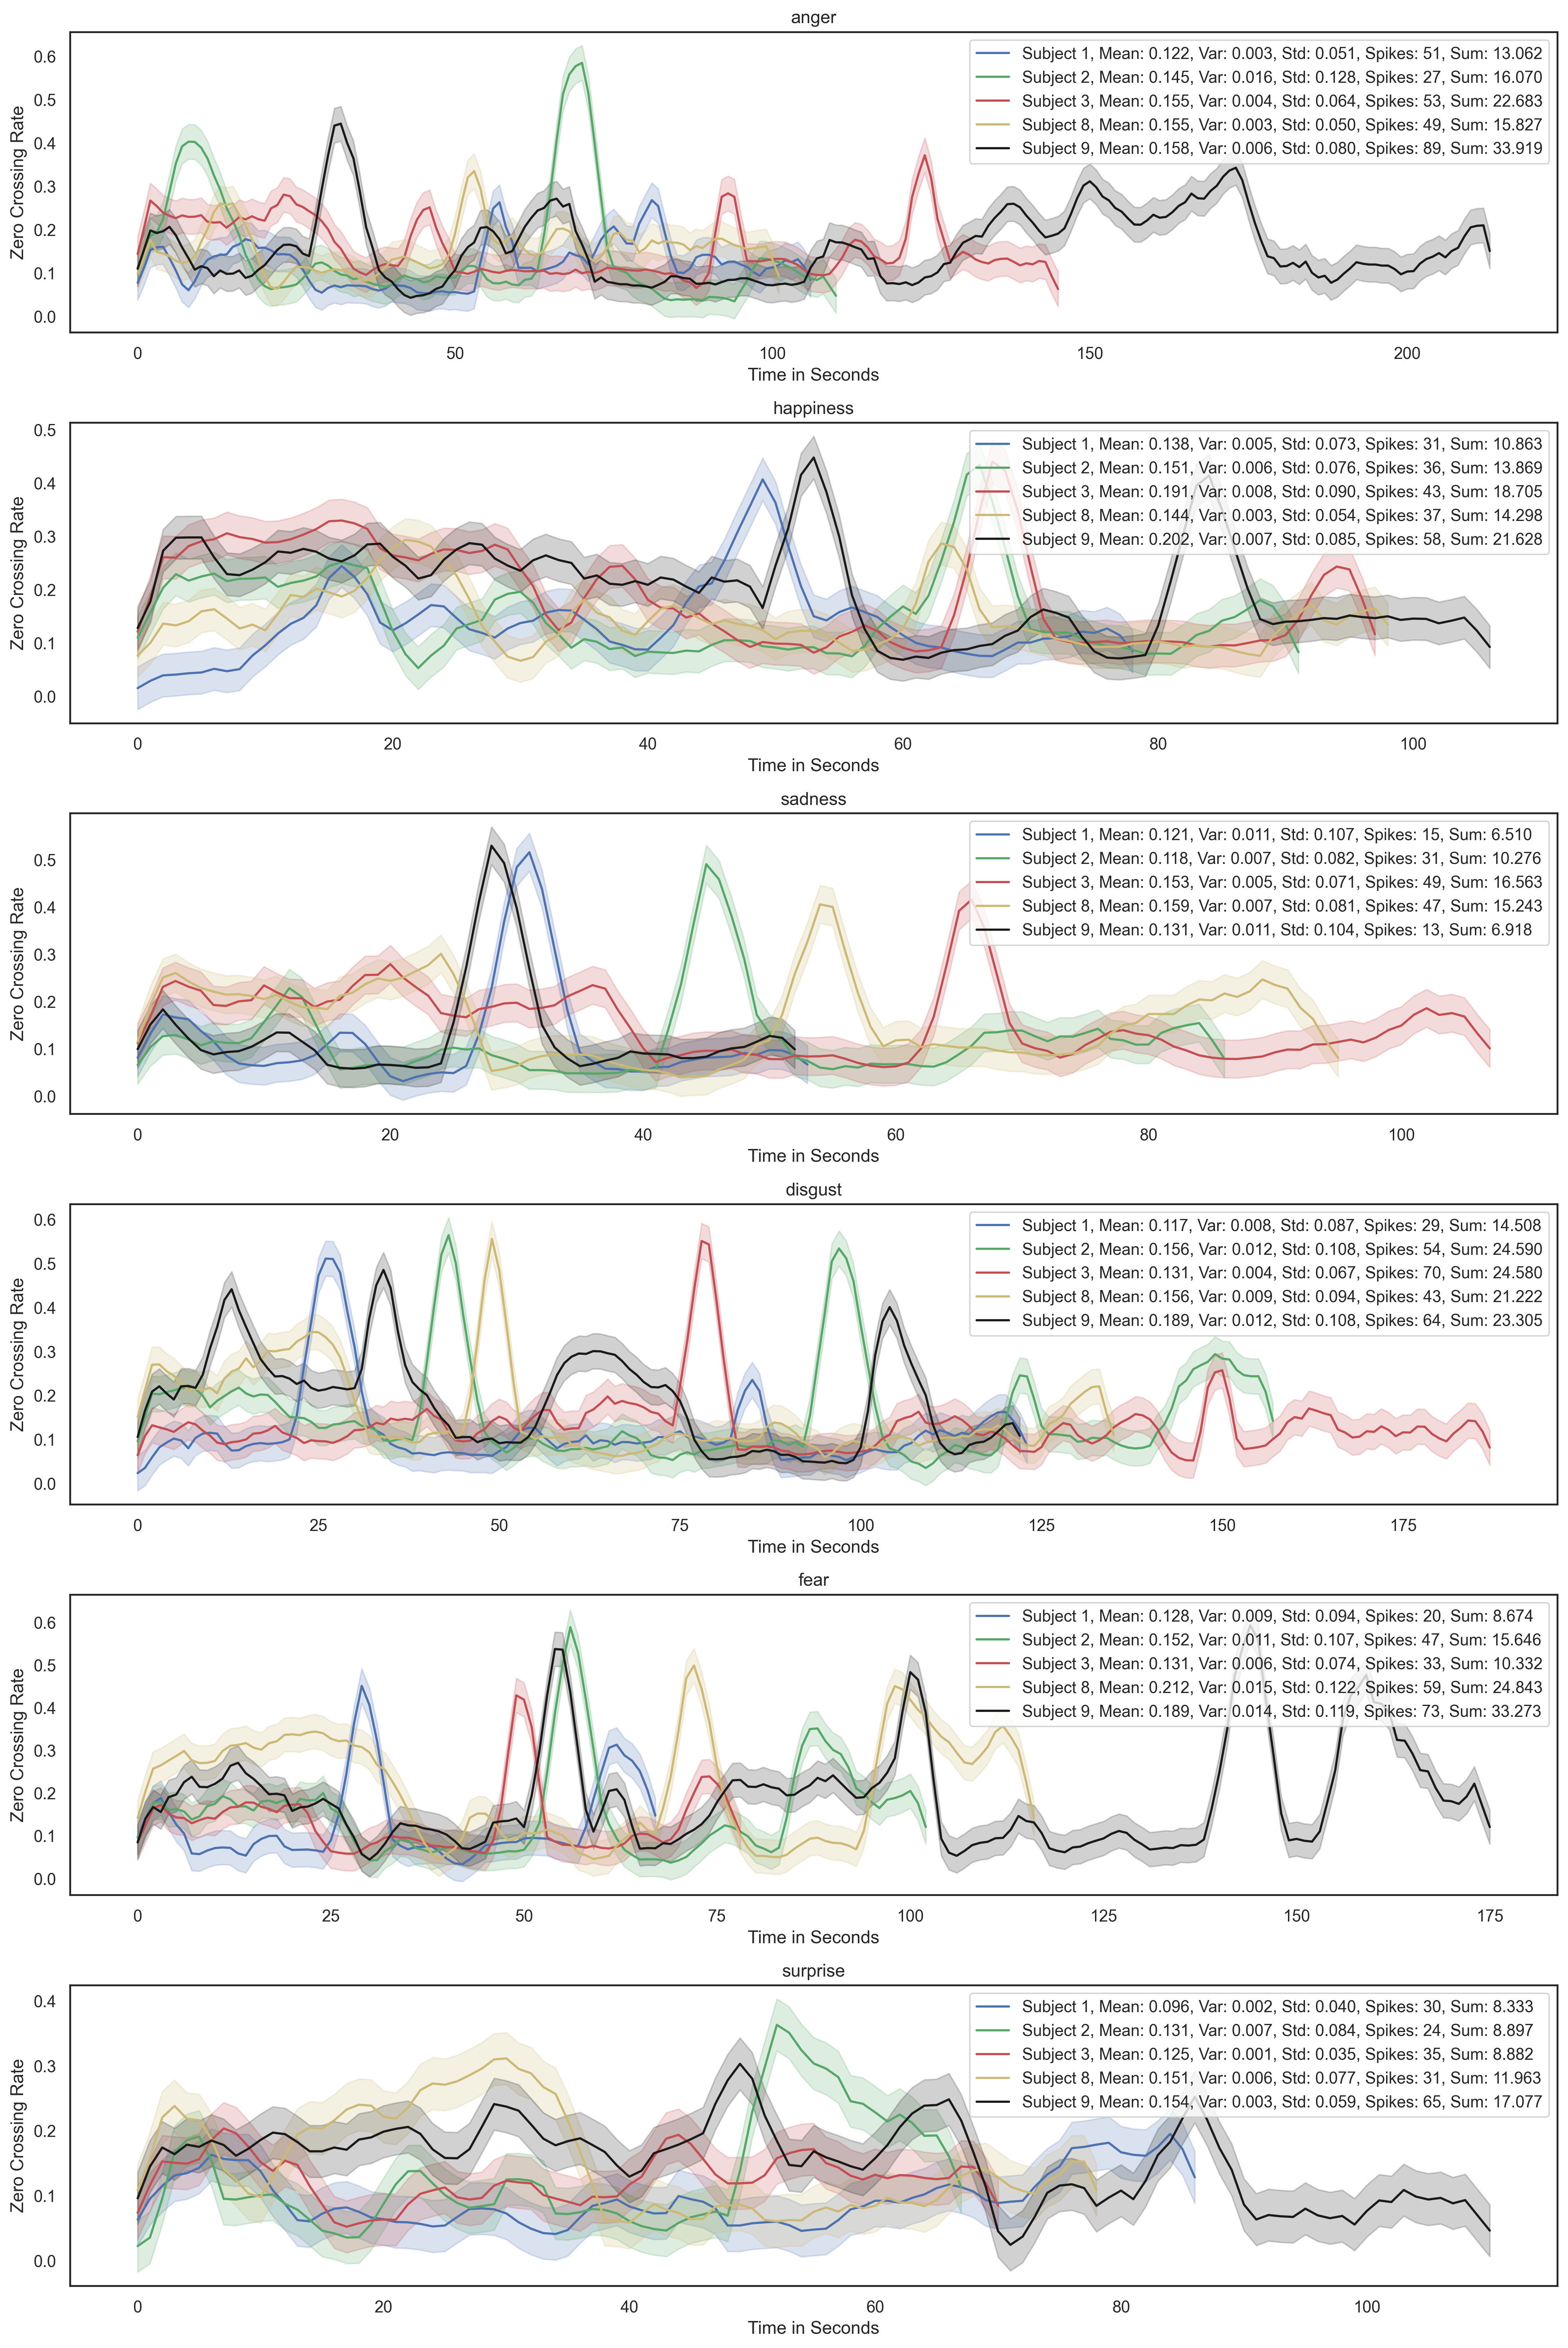
\includegraphics[width=.8\linewidth]{figs/appendix/feature_selection/zcrArea.png}
	\caption{Zero Crossing Rate Wave Plots with a Surrounding Area of Five Male Subjects and the same Sentence for All Emotions}
	\label{fig:zcrArea}
\end{figure}

\section{Feature Variation Plots}

\begin{figure}[H]
	\centering
	\includegraphics[width=.8\linewidth]{figs/appendix/feature_selection/stdZCRVar.png}
	\caption{Zero crossing rate standard deviation values variation plot along 50 audios of speech utterances for all emotions}
	\label{fig:stdZCRVar}
\end{figure}

\begin{figure}[H]
	\centering
	\includegraphics[width=.8\linewidth]{figs/appendix/feature_selection/spikesZCRVar.png}
	\caption{Zero crossing rate spikes values variation plot along 50 audios of speech utterances for all emotions}
	\label{fig:spikesZCRVar}
\end{figure}

\begin{figure}[H]
	\centering
	\includegraphics[width=.8\linewidth]{figs/appendix/feature_selection/sumZCRVar.png}
	\caption{Zero crossing rate sum values variation plot along 50 audios of speech utterances for all emotions}
	\label{fig:sumZCRVar}
\end{figure}



\section{Confusion Matrices}  \label{confusionMatrices}

\begin{figure}[H]
	\centering
	\includegraphics[width=.55\linewidth]{figs/appendix/feature_selection/cmAll.png}
	\caption{Confusion Matrix of a Ridge Classifier Trained using all 327 Extracted Features}
	\label{fig:confMatrix1}
\end{figure}

\begin{figure}[H]
	\centering
	\includegraphics[width=.55\linewidth]{figs/appendix/feature_selection/cmSec.png}
	\caption{Confusion Matrix of a Ridge Classifier Trained using 97 Features After High Correlation Feature Elimination}
	\label{fig:confMatrix2}
\end{figure}


\begin{figure}[H]
	\centering
	\includegraphics[width=.55\linewidth]{figs/appendix/feature_selection/cmThird.png}
	\caption{Confusion Matrix of a Ridge Classifier Trained using 35 Features After High Correlation and Backward Selection}
	\label{fig:confMatrix3}
\end{figure}


\begin{figure}[H]
	\centering
	\includegraphics[width=.55\linewidth]{figs/appendix/feature_selection/AdaBoostCM.png}
	\caption{Confusion Matrix of an AdaBoost Classifier.}
\end{figure}

\begin{figure}[H]
	\centering
	\includegraphics[width=.55\linewidth]{figs/appendix/feature_selection/RandomForestCM.png}
	\caption{Confusion Matrix of a Random Forest Classifier.}
\end{figure}

\begin{figure}[H]
	\centering
	\includegraphics[width=.55\linewidth]{figs/appendix/feature_selection/HistCM.png}
	\caption{Confusion Matrix of a Histogram Gradient Boosting Classifier.}
\end{figure}

\begin{figure}[H]
	\centering
	\includegraphics[width=.55\linewidth]{figs/appendix/feature_selection/BalancedForestCM.png}
	\caption{Confusion Matrix of a Balanced Random Forest Classifier.}
\end{figure}

\begin{figure}[H]
	\centering
	\includegraphics[width=.55\linewidth]{figs/appendix/feature_selection/LSTMCM.png}
	\caption{Confusion Matrix of a \ac{lstm} Classifier.}
\end{figure}

\begin{figure}[H]
	\centering
	\includegraphics[width=.55\linewidth]{figs/appendix/feature_selection/CNNCM.png}
	\caption{Confusion Matrix of a \ac{cnn} Classifier.}
\end{figure}

\begin{figure}[H]
	\centering
	\includegraphics[width=.55\linewidth]{figs/appendix/feature_selection/LDACM.png}
	\caption{Confusion Matrix of a Linear Discriminant Analysis Classifier.}
\end{figure}

\begin{figure}[H]
	\centering
	\includegraphics[width=.55\linewidth]{figs/appendix/feature_selection/RidgeCM.png}
	\caption{Confusion Matrix of a Ridge Classifier.}
\end{figure}



\section{Something else}

\begin{figure}[H]
	\centering
	\includegraphics[width=1\linewidth]{figs/appendix/IEMOCAP_data_study/activationScatterAllEmotions.png}
	\caption{Scatter Plot of the Annotated Emotions in the Activation Dimension}
	\label{fig:activationScatter}
\end{figure}

\begin{figure}[H]
	\centering
	\includegraphics[width=1\linewidth]{figs/appendix/IEMOCAP_data_study/dominanceScatterAllEmotions.png}
	\caption{Scatter Plot of the Annotated Emotions in the Dominance Dimension}
	\label{fig:dominanceScatter}
\end{figure}


\begin{figure}[H]
	\centering
	\includegraphics[width=1\linewidth]{figs/appendix/IEMOCAP_data_study/neutralScatterViolins.png}
	\caption{Scatter and violin plots of the emotional content of the IEMOCAP corpus in terms of valence, activation, and dominance relative to the neutral emotion}
	\label{fig:neutralScatterViolins}
\end{figure}


\begin{figure}[H]
	\centering
	\includegraphics[width=1\linewidth]{figs/appendix/IEMOCAP_data_study/sadScatterViolins.png}
	\caption{Scatter and violin plots of the emotional content of the IEMOCAP corpus in terms of valence, activation, and dominance relative to the sad emotion}
	\label{fig:sadScatterViolins}
\end{figure}


\begin{figure}[H]
	\centering
	\includegraphics[width=1\linewidth]{figs/appendix/IEMOCAP_data_study/happyScatterViolins.png}
	\caption{Scatter and violin plots of the emotional content of the IEMOCAP corpus in terms of valence, activation, and dominance relative to the happiness emotion}
	\label{fig:happyScatterViolins}
\end{figure}


